%File: formatting-instruction.tex
\documentclass[letterpaper]{article}
\usepackage{aaai}
\usepackage{times}
\usepackage{helvet}
\usepackage{courier}
\usepackage{graphicx}
\frenchspacing
\setlength{\pdfpagewidth}{8.5in}
\setlength{\pdfpageheight}{11in}
\pdfinfo{
/Title (Insert Your Title Here)
/Author (Put All Your Authors Here, Separated by Commas)}
\setcounter{secnumdepth}{0}  
 \begin{document}
% The file aaai.sty is the style file for AAAI Press 
% proceedings, working notes, and technical reports.
%
\title{Trading Cryptocurrencies with\\Reinforcement Learning}
\author{University of Colorado Colorado Springs\\Jacob Quatkemeyer\\Caden Aragon
}
\maketitle
\begin{abstract}
\begin{quote}
People have been trading stocks on the stock market since the early 1800's. Stock trading is a complicated, but potentially very profitable way of making money. Another way to find great
profit, or loss, is by trading cryptocurrencies. Cryptocurrencies, much like stocks, vary in their price each and every second, and people buy and sell these coins hoping to make a profit. There are many styles of trading, including scalping, day trading, intraday trading, etc. While many have been successful using these traditional trading techniques, this paper looks to explore reinforcement learning and deep reinforcement learning to optimize a cryptocurrency trading strategy that can outperform a human trader.
\end{quote}
\end{abstract}

\section{1 Introduction}
\noindent The first official cryptocurrency was Bitcoin, which was established in 2009. Each "coin" started trading at as low as \$0.008 per coin. Just over a twelve years later, a single Bitcoin reached the price of \$64,863. Many people who invested early made millions of dollars, while other investors may have lost fortunes. The problem with trading and investing in cypto coins is that it is mostly a gamble. Although there are different patterns a trader can learn to recognize to predict the movement in the market, this is unreliable and limited. A possible solution to combat human limitations is to train an agent to read market indicators and recognize patterns using reinforcement learning.

Vital to the prediction of cryptocurrency movement are the large amount of indicators. Some of the most popular indicators include the relative strength index (RSI), Bollinger bands, moving average convergence divergence (MACD), and many others. A successful trading bot would be able to read multiple indicators, and recognize patterns that would allow it to predict the movement of the coin on the market, and idealy lead to profit. 

Another issue with trading coins manually is the frequency in which you can trade coins. A trader has to read different indicators for different coins. A human trader is limited to trading a smaller number of coins for longer. Computers, even without the use of reinforcment learning, can read the indicators and trade dozens of coins at a time. This is known as high frequency trading (HFT). This technique of trading involves holding many positions at a time, and earning a very small profit on a large number of transactions, leading to a sizeable profit (Huang, Huan, Xu, Zheng, \& Zou, 2019).

Other papers have tried to use different reinforcement learning algorithms to trade coins frequently with different indicators, but the majority of researchers train their agent with either many indicators on a few coins, or even no indicators on one coin. They also tend to test only one algorithm, and measure them against the algorithms used by other researchers. In this paper, we aim to find a good mix between valuable indicators, heavily traded coins, and different algorithms to trade our agent with. We start with a simple Q learning algorithm, to see its limitations, and move on to a Deep Q algorithm using a neural network. The goal is to train our agent well enough to outperform human traders on the cryptocurrency trading market, and to see what kind of limitations different algorithms have.

\section{2 Background}
Reinforcement learning is.... (short history, definition, common uses etc.)
... Cryptocurrencies have a large amount if indicators and values that can depict a state, so the state space can become very large, and we would need a huge amount of data to train an agent. Because of this, we would like to try and implement a Monte Carlo learning algorithm and measure the effectiveness, or lack thereof. We then will compare it to an algorithm that uses a neural network to accomplish it's training, a much better suited technique for tackling such a huge problem.
\subsection{2.1}
Q learning is...(cite papers to define monte carlo, its pros, cons, etc.)...

\subsection{2.2} 
Deep Q learning is....(definition, the fact that it uses neural networks, etc.)

\section{3 Related Work}
Give short summary on the paper (Jae Won Lee, "Stock price prediction using reinforcement learning," ISIE 2001. 2001 IEEE International Symposium on Industrial Electronics Proceedings (Cat. No.01TH8570), 2001, pp. 690-695 vol.1, doi: 10.1109/ISIE.2001.931880.) which is on using temporal-difference algorithms with a neural network.

\section{4 Methodology}
We will begin by training the agent on historical cryptocurrency trading data from multiple different coins using a Q learning algorithm. Training the data on different coins will avoid generalization and will give the agent a greater range of data to learn from. Each time step of the data will be measured by the hour to take advantage of the 24 hour market that cryptocurrencies are sold on. The market is volatile enough to still make a prophet using one hour time steps. We will then test the agent on a different range of data, again from multiple different coins, to find out how profitable and reliable the Q learning trained agent is for automated trading. Our next step is to train a new agent using a Deep Q learning algorithm, taking advantage of a multi-layered neural network. We will train this agent in the exact same way we trained the first. However, depending on the efficiency of this new algorithm, we may give it more data to train on.
\subsection{4.1 Data}
To get a range of data, we will be using an API from the exchange known as Binance. This API will allow us to download any range of data from any coin on its market. It is a useful tool that we could implement into the training network, allowing the training program to dynamically download more data to learn from based on different parameters.
\subsection{4.2 Training}
We will be training the agents using the basics behind many Reinforcement Learning training algorithms. We first define the state space. A state at any given time step will include a number of cryptocurrency trading indicators. The amount of indicators will depend on the efficiency of each trading algorithm because the larger amount of indicators will provide us with a bigger Q-Table, requiring more processing power. In general, we will use the as many of the most commonly used indicators in trading that the algorithm can effecitively handle. The action space is defined very simply, with only three actions: buy, sell, and hold. The agent will be rewarded positively for the amount of profit at the end of each day. The more profit, the more reward. The agent will be rewarded negatively for each loss. Again, the great the loss, the greater the punishment.

\section{5 Evaluation}
The two agents will be evaluated with two values, profit and the Sharpe ratio. The Sharpe ratio is defined:
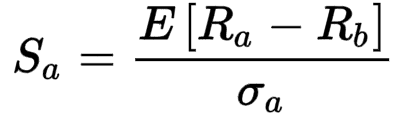
\includegraphics{Sharpe} 
\\
\\
where
\[ R_a = asset\ return \] 
\[ R_b = risk\ free\ return \] 
\[ E = expected\  value \] 
\[ \sigma_a = standard\ deviation\ of\ the\ asset\ excess\ return \] 

The Sharpe ratio tells the expected profit when accounting for loss. A portfolio can earn 100\% profit one month and seem like its an incredibly profitable strategy. However, if it loses 100\% for the next six months, then that means the trading strategy, or in our case the agents policy, is not efficiently profitable, it just happened to get lucky during the first month. Profit is important, but only if the risk is also calculated. We will evaluate the Sharpe ratio that each agent is capable of earning to ensure that the agent profits without risking too much of its assets.
	
\section{6 Timeline}

\section{7 Conclusion}

\section{References}
\smallskip \noindent \textit{B. Huang, Y. Huan}\\
Automated trading systems statistical and machine learning methods and hardware implementation: A survey Enterprise Information Systems, L.D. Xu, L. Zheng, Z. Zou 2019. \textit{Blackboard Systems.} 13 (1) (2019), pp. 132-144
B. Huang, Y. Huan


\end{document}
